\chapter{CPDAG}

\section{PDAGs}

\begin{definition}[PDAG]
    An acyclic partially directed graph, or PDAG for short, is a graph that contains both directed and undirected edges. It is acyclic in the sense that it contains no directed cycles.
\end{definition}
\begin{remark}
    An acyclic directed graph, or DAG for short, can be regarded as a PDAG without undirected edges.
\end{remark}
Here we list some graph theoretical concepts for a PDAG.
\begin{itemize}
    \item The \textit{skeleton} of any PDAG is the undirected graph resulting from ignoring the directionality of every edge. 
    \item A \textit{v-structure} in a PDAG $\cG$ is an ordered triple of nodes $(x,y,z)$ such that $\cG$ contains the directed edges $x \rightarrow y$ and $z \rightarrow y$, and $x$ and $z$ are not adjacent in $\cG$.
    \item A \textit{clique} in a PDAG is a set of nodes for which every pair of nodes is adjacent.
\end{itemize}
We also list some notations for a PDAG.
\begin{itemize}
    \item We use $\Pi_x$ to denote the set of parents for node $x$ in a PDAG.
    \item We use $N_x$ to denote the set of neighbors of node $x$ in a PDAG.
    \item We use $N_{x,y} = N_x \cap N_y$ to denote the set of common neighbors of $x$ and $y$ in a PDAG.
    \item We use $\Omega_{x,y} = \Pi_x \cap N_y$ to denote the set of parents of node $x$ that are neighbors of node $y$ in a PDAG.
    %\item We say a directed edge $x \rightarrow y$ is \textit{covered} if $\Pi_x = \Pi_y \setminus x$. Similarly, we say an undirected edge is covered if $ \Pi_x = \Pi_y$.
\end{itemize}

\section{MECs}

Two network structures are equivalent if the set of distributions that can be represented using one of the structures is identical to the set of distributions that can be represented using the other.
\begin{theorem}\label{thm:verma}
    Two DAGs are Markov equivalent if and only if they have the same skeleton and the same v-structures.
\end{theorem}
\begin{proof}
    
\end{proof}


\begin{definition}[CPDAG]
    The CPDAG of a DAG $\cD$, denoted as $\cC$, is a PDAG that has the same skeleton as $\cD$, and an edge is directed in $\cC$ if and only if it has the same orientation in every equivalent DAG of $\cD$.
\end{definition}
We can distinguish two kinds of edges in a DAG according to its CPDAG. A directed edge of a DAG is \textit{compelled} if it occurs in the corresponding CPDAG, otherwise, the directed edge is \textit{reversible}, and the corresponding parents are reversible parents.

\section{A Transformational Characterization of MECs}
\begin{definition}
    A directed edge $x\rightarrow y$ is \textit{covered} if $\Pi_{y}=\Pi_{x}\cup\{x\}$.
\end{definition}

\begin{theorem}\label{thm:transformational}
    Let $\cG$ be any DAG containing the edge $x \rightarrow y$, and let $\cG'$ be the directed graph identical to $\cG$ except that the edge between $x$ and $y$ in $\cG'$ is oriented as $y\rightarrow x$. Then $\cG'$ is a DAG that is equivalent to $\cG$ if and only if $x\rightarrow y$ is a covered edge in $\cG$.
\end{theorem}


\section{Characterization of CPDAGs}
We introduce some terminologies and the main theorem.
\begin{itemize}
    \item A PDAG is called a \textit{chain graph} if it contains no semi-directed cycles.
    \item An undirected graph is \textit{chordal} if every cycle of length greater than or equal to 4 possesses a chord.
    \item A directed edge $v\rightarrow u$ in a PDAG $\cP$ is \textit{strongly protected} if $v\rightarrow u$ occurs in at least one of the four induced subgraphs of $\cP$ in Figure \ref{fig:stronglyprotected}.
\end{itemize}

\begin{figure}[h]
    \caption{Configurations where $v \rightarrow u$ is strongly protected.}
    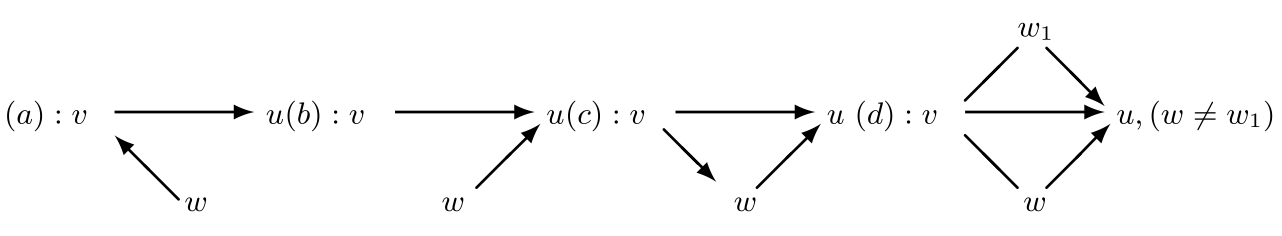
\includegraphics[width=\textwidth]{strongly protected.png}
    \label{fig:stronglyprotected}
\end{figure}


\begin{theorem}
    A graph $\cC$ is a CPDAG of a directed acyclic graph $\cD$ if and only if $\cC$ satisfies the following properties:
    \begin{enumerate}
        \item $\cC$ is a chain graph;
        \item let $\cC_\tau$ be the subgraph induced by $\tau$. $\cC_\tau$ is chordal for every chain component $\tau$;
        \item $w \rightarrow u - v$ does not occur as an induced subgraph of $\cC$;
        \item every arrow $v \rightarrow u$ in $\cC$ is strongly protected.
    \end{enumerate}
\end{theorem}
\begin{remark}
    
\end{remark}

The following series of lemma closely inspect a clique of size three in a CPDAG $\cC$, where there exists an undirected edge

\begin{lemma}\label{lem:0.4.1}
    The configuration $w \rightarrow u - v$ does not occur as an induced subgraph of $\cC$.
\end{lemma}
\begin{proof}
    If $w \rightarrow u - v$ occurs as an induced subgraph in $\cC$, then $w \rightarrow u \leftarrow v$ must occurs as a v-structure in some $\cD\sim\text{Class}(\cC)$. By Theorem \ref{thm:verma}, this is impossible.
\end{proof}



\begin{lemma}\label{lem:0.4.2}
    If 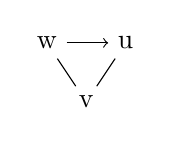
\begin{tikzpicture}[scale=0.5]
        % Nodes
        \node (w) at (0,0) {w};
        \node (u) at (2,0) {u};
        \node (v) at (1,-1.5) {v};
      
        % Edges
        \draw[->] (w) -- (u);
        \draw (v) -- (w);
        \draw (v) -- (u);
      \end{tikzpicture} 
      occurs in $\cC$, then there exist $\cD_1,\cD_2\in \text{Class}(\cC)$ such that 
      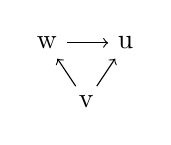
\begin{tikzpicture}[scale=0.5]
        % Nodes
        \node (w) at (0,0) {w};
        \node (u) at (2,0) {u};
        \node (v) at (1,-1.5) {v};
      
        % Edges
        \draw[->] (w) -- (u);
        \draw[->] (v) -- (w);
        \draw[->] (v) -- (u);
      \end{tikzpicture} occurs in $\cD_1$ and 
      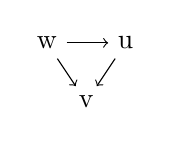
\begin{tikzpicture}[scale=0.5]
        % Nodes
        \node (w) at (0,0) {w};
        \node (u) at (2,0) {u};
        \node (v) at (1,-1.5) {v};
      
        % Edges
        \draw[->] (w) -- (u);
        \draw[->] (w) -- (v);
        \draw[->] (u) -- (v);
      \end{tikzpicture} occurs in $\cD_2$.
\end{lemma}
\begin{proof}
    Any $\cD\in\cls(\cC)$ must contain one of the followings:
    \[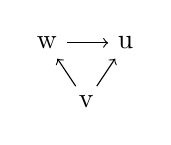
\begin{tikzpicture}[scale=0.5]
        % Nodes
        \node (w) at (0,0) {w};
        \node (u) at (2,0) {u};
        \node (v) at (1,-1.5) {v};
      
        % Edges
        \draw[->] (w) -- (u);
        \draw[->] (v) -- (w);
        \draw[->] (v) -- (u);
      \end{tikzpicture},\quad 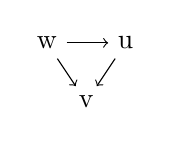
\begin{tikzpicture}[scale=0.5]
        % Nodes
        \node (w) at (0,0) {w};
        \node (u) at (2,0) {u};
        \node (v) at (1,-1.5) {v};
      
        % Edges
        \draw[->] (w) -- (u);
        \draw[->] (w) -- (v);
        \draw[->] (u) -- (v);
      \end{tikzpicture}, \quad 
      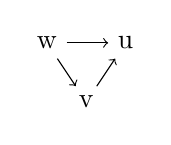
\begin{tikzpicture}[scale=0.5]
        % Nodes
        \node (w) at (0,0) {w};
        \node (u) at (2,0) {u};
        \node (v) at (1,-1.5) {v};
      
        % Edges
        \draw[->] (w) -- (u);
        \draw[->] (w) -- (v);
        \draw[->] (v) -- (u);
      \end{tikzpicture}.\]
    
\end{proof}

\begin{lemma}\label{lem:0.4.3}
    Let $\{w, u, v\}$ be any three nodes that form a clique of size three in $\cC$. If any two of the edges in the clique are undirected, then the third edge is undirected as well.
\end{lemma}
\begin{proof}
    Assume 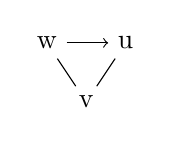
\begin{tikzpicture}[scale=0.5]
        % Nodes
        \node (w) at (0,0) {w};
        \node (u) at (2,0) {u};
        \node (v) at (1,-1.5) {v};
      
        % Edges
        \draw[->] (w) -- (u);
        \draw (v) -- (w);
        \draw (v) -- (u);
      \end{tikzpicture} occurs in $\cC$, we prove by contradiction. 
      According to Lemma \ref*{lem:0.4.2}, suppose 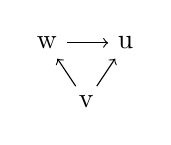
\begin{tikzpicture}[scale=0.5]
        % Nodes
        \node (w) at (0,0) {w};
        \node (u) at (2,0) {u};
        \node (v) at (1,-1.5) {v};
      
        % Edges
        \draw[->] (w) -- (u);
        \draw[->] (v) -- (w);
        \draw[->] (v) -- (u);
      \end{tikzpicture} occurs in $\cD_1$ and 
      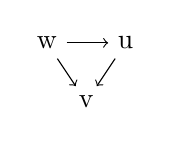
\begin{tikzpicture}[scale=0.5]
        % Nodes
        \node (w) at (0,0) {w};
        \node (u) at (2,0) {u};
        \node (v) at (1,-1.5) {v};
      
        % Edges
        \draw[->] (w) -- (u);
        \draw[->] (w) -- (v);
        \draw[->] (u) -- (v);
      \end{tikzpicture} occurs in $\cD_2$. \par
      As $w\rightarrow u$ is compelled, applying Theorem \ref{thm:transformational} to $\cD_1$ yields that $w\to u$ is not a covered edge in $\cD_1$.
      Therefore, there exists $x$ such that $x$ is a parent of $u$ but not a parent of $w$ in $\cG$. Now consider the subgraph induced by $\{u,v,w,x\}$ in $\cD_1$.
      If there is no edge between $x$ and $v$, then $x\rightarrow u \leftarrow v$ forms a v-structure, which is impossible. So there must be an edge between $x$ and $v$.\par 
      Now consider the subgraph induced by $\{u,v,w,x\}$ in $\cD_2$. As $x\rightarrow u \leftarrow w$ forms a v-structure in $\cD_1$, it also forms a v-structure in $\cD_2$ by Theorem \ref{thm:verma}. 
      Moreover, there must be an edge between $x$ and $v$. If $v\to x$, then $\cD_2$ contains a directed cycles. If $x\rightarrow v$ in $\cD_2$, then $x\rightarrow v \leftarrow w$ forms a v-structure, which is also impossible.

\end{proof}

\begin{lemma}\label{lem:0.4.4}
    Suppose there is a directed path from $v$ to $u$ in $\cC$. If there is an edge between $v$ and $u$, then it must be $v \rightarrow u$.
\end{lemma}
\begin{proof}
    Any $\cD\in\cls(\cC)$ must be acyclic.
\end{proof}

\begin{corollary}\label{cor:0.4.1.1}
    If $u - v$ is an undirected edge in $\cC$, then $\Pi_u = \Pi_v$.
\end{corollary}
\begin{proof}
    Suppose not. Without loss of generality, let $w$ be any parent of $u$ that is not a parent of $v$. 
    There are three configuration of the subgraph induced by $\{u,v,w\}$ in general: 
    \[\begin{tikzpicture}[scale=0.5]
        % Nodes
        \node (w) at (0,0) {w};
        \node (u) at (2,0) {u};
        \node (v) at (1,-1.5) {v};
      
        % Edges
        \draw[->] (w) -- (u);
        \draw (u) -- (v);
      \end{tikzpicture},\quad
    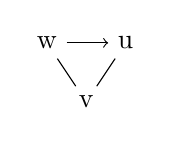
\begin{tikzpicture}[scale=0.5]
        % Nodes
        \node (w) at (0,0) {w};
        \node (u) at (2,0) {u};
        \node (v) at (1,-1.5) {v};
      
        % Edges
        \draw[->] (w) -- (u);
        \draw (w) -- (v);
        \draw (u) -- (v);
      \end{tikzpicture},\quad
      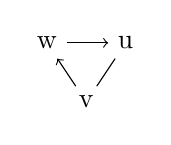
\begin{tikzpicture}[scale=0.5]
        % Nodes
        \node (w) at (0,0) {w};
        \node (u) at (2,0) {u};
        \node (v) at (1,-1.5) {v};
      
        % Edges
        \draw[->] (w) -- (u);
        \draw[->] (v) -- (w);
        \draw (u) -- (v);
      \end{tikzpicture}.\]
      The first case is excluded by Lemma \ref*{lem:0.4.1}, the second case is excluded by Lemma \ref*{lem:0.4.3}, and the third case is excluded by Lemma \ref*{lem:0.4.4}.
\end{proof}

Next we focus on the chain graph structure, \emph{i.e.} maximal undirected components in $\cC$.
A maximal undirected component $K$ of a CPDAG $\cC$ is a connected subgraph of $\cC$, where each connecting edge is undirected, and for every node $x \in K$, if there is an undirected edge $y-x$ in $\cC$, then $y\in K$.
For the remainder of this note, we use \textit{undirected component} to mean maximal undirected component.

\begin{lemma}\label{lem:0.4.6}
    For any directed edge $u \rightarrow v$ in $\cC$, $u$ is a parent of every node reachable by $v$ via undirected edges.
\end{lemma}
\begin{proof}
    Follows by a repeated application of Corollary \ref*{cor:0.4.1.1} along the edges in any undirected path.
\end{proof}

\begin{lemma}\label{lem:0.4.7}
    If there is a directed path of length one or more from $u$ to $v$ in $\cC$, then $u$ and $v$ are not in the same undirected component.
\end{lemma}
\begin{proof}
    Suppose not. Consider the last edge $w \rightarrow v$ in the directed path. By Lemma \ref*{lem:0.4.6}, $w$ is a parent of every node in the undirected component containing $v$, which means that $w$ is a parent of $u$. This forms a cycle.
\end{proof}

The next lemma shows that the undirected components of a CPDAG are chordal.
\begin{lemma}\label{lem:0.4.5}
    $\cC$ has no undirected chordless $k$-cycles $(k\geq 4)$.
\end{lemma}
\begin{proof}
    If an undirected chordless $k$-cycle occurs in $\cC$, then $\cC$ must have at least one v-structure in this cycle.
\end{proof}

\begin{corollary}
    Let $u$ and $v$ be any pair of nodes that are not adjacent in $\cC$. Then $N_{x,y}$ is a clique of undirected edges.
\end{corollary}

Now we consider the converse of Corollary \ref*{cor:0.4.1.1}.

\begin{lemma}
    If $v\rightarrow u$ is a directed edge in $\cC$, then $\Pi_u\neq \Pi_v\cup\{v\}$.
\end{lemma}
\begin{proof}
    
\end{proof}


\begin{lemma}
    Every directed edge $v\rightarrow u$ in $\cC$ is strongly protected.
\end{lemma}
\begin{proof}
    According to Lemma, we only need to show that if 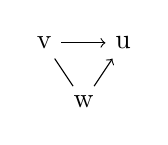
\begin{tikzpicture}[scale=0.5]
        % Nodes
        \node (w) at (0,0) {v};
        \node (u) at (2,0) {u};
        \node (v) at (1,-1.5) {w};
      
        % Edges
        \draw[->] (w) -- (u);
        \draw[->] (v) -- (u);
        \draw (v) -- (w);
      \end{tikzpicture} occurs in $\cC$, then the configuration (d) in Figure \ref{fig:stronglyprotected} occurs as an induced subgraph.
\end{proof}

Now we begin the proof of Theorem 
\begin{proof}
    We first prove the only if direction.
\end{proof}



\section{Algorithm: }


\section{Algorithm: }

\begin{definition}
    An operator is valid if
    \begin{itemize}
        \item the modified graph of the operator is a PDAG and has a consistent extension;
        \item 
    \end{itemize}
\end{definition}

\subsection{Compelled and Reversible Edge Insertions}
\begin{theorem}\label{thm:0.7.1}
    Let $\cC$ be any CPDAG for which nodes $x$ and $y$ are not adjacent. If the result of adding an edge between $x$ and $y$ is a PDAG that admits a consistent extension, then that edge is compelled if and only if $\Pi_x \neq \Pi_y$.
\end{theorem}
One reason that Theorem \ref*{thm:0.7.1} is difficult to prove is that after inserting edges into a CPDAG, edges that were reversible before can become compelled, and edges that were compelled before can become reversible.
In the following lemmas, we demonstrate a method for determining which edges in a CPDAG will necessarily remain compelled and reversible after an edge addition, based on the topology of the CPDAG.

\begin{lemma}
    Let $\cC$ be a CPDAG,and let $\cP$ denote the PDAG that results from an edge addition or deletion. If $\cP$ admits a consistent extension, then any compelled edge $x \rightarrow y$ in $\cC$ cannot be compelled in the opposite direction in $\cP$.
\end{lemma}
\begin{proof}
    
\end{proof}

\subsection{The InsertU Operator}
\begin{theorem}
    Let $x$ and $y$ be two nodes that are not adjacent in $\cC$. The insertion of the undirected edge $x - y$ is valid if and only if (1) every undirected path between $x$ and $y$ contains a node in $N_{x,y}$, and (2) $\Pi_x = \Pi_y$.
\end{theorem}

\subsection{The DeleteU Operator}
\begin{theorem}
    Let $x - y$ be an undirected edge in CPDAG $\cC$. The deletion of $x - y$ is valid if and only if $N_{x,y}$ is a clique of undirected edges.
\end{theorem}

\subsection{The InsertD Operator}
\begin{lemma}
    Let $\cC$ be a CPDAG that contains a semi-directed path from $x$ to $y$. If there exists a directed edge $z \rightarrow w$ in this path, then there exists a directed path from $z$ to $y$ in $\cC$.
\end{lemma}

\begin{theorem}
    Let $x$ and $y$ be any two nodes that are not adjacent in CPDAG $\cC$. The insertion of $x \rightarrow y$ is valid if and only if (1) every semi-directed path from $y$ to $x$ contains at least one node in $\Omega_{x,y}$, (2) $\Omega_{x,y}$ is a clique of undirected edges, and (3) $\Pi_x \ne \Pi_y$.
\end{theorem}

\subsection{The DeleteD Operator}
\begin{theorem}
    Let $x \rightarrow y$ be a directed edge in CPDAG $\cC$. The deletion of $x \rightarrow y$ is valid if and only if $N_y$ is a clique of undirected edges.
\end{theorem}

\subsection{The ReverseD Operator}
\begin{theorem}
    Let $x \rightarrow y$ be a directed edge in CPDAG $\cC$. The reversal of $x \rightarrow y$ is valid if and only if (1) every semi-directed path from $x$ to $y$ that does not include the edge $x \rightarrow y$ contains at least one node in $\Omega_{y,x} \cup N_y$, and (2) $\Omega_{y,x}$ is a clique of undirected edges.
\end{theorem}

\subsection{The MakeV Operator}
\begin{theorem}
    Let $x - z - y$ be any length-two undirected path in CPDAG $\cC$ such that x and y are not adjacent. Replacing the undirected edges with directed edges to create the v-structure $x \rightarrow z \leftarrow y$ is valid if and only if every undirected path between $x$ and $y$ contains a node in $N_{x,y}$.
\end{theorem}

\section{Algorithm: Reversible MCMC on MECs}

We need to show each operator has a reversible operator.

\subsection{The InsertU Operator}
\begin{theorem}
    Let $x$ and $y$ be two nodes that are not adjacent in $\cC$. The insertion of the undirected edge $x - y$ is reversible if and only if (1) every undirected path between $x$ and $y$ contains a node in $N_{x,y}$, and (2) $\Pi_x = \Pi_y$.
\end{theorem}

\subsection{The DeleteU Operator}
\begin{theorem}
    Let $x - y$ be an undirected edge in CPDAG $\cC$. The deletion of $x - y$ is valid if and only if $N_{x,y}$ is a clique of undirected edges.
\end{theorem}

\subsection{The InsertD Operator}
\begin{lemma}
    Let $\cC$ be a CPDAG that contains a semi-directed path from $x$ to $y$. If there exists a directed edge $z \rightarrow w$ in this path, then there exists a directed path from $z$ to $y$ in $\cC$.
\end{lemma}

\begin{theorem}
    Let $x$ and $y$ be any two nodes that are not adjacent in CPDAG $\cC$. The insertion of $x \rightarrow y$ is valid if and only if (1) every semi-directed path from $y$ to $x$ contains at least one node in $\Omega_{x,y}$, (2) $\Omega_{x,y}$ is a clique of undirected edges, and (3) $\Pi_x \ne \Pi_y$.
\end{theorem}

\subsection{The DeleteD Operator}
\begin{theorem}
    Let $x \rightarrow y$ be a directed edge in CPDAG $\cC$. The deletion of $x \rightarrow y$ is valid if and only if $N_y$ is a clique of undirected edges.
\end{theorem}


\subsection{The RemoveV Operator}
First we show that RemoveC is valid.
\begin{theorem}
    
\end{theorem}

Next we show that RemoveC is reversible.

\section{Counting Sizes of MECs}
\subsection{Size of MEC Determined by the Number of Vertices}
Let $\cU_{p,n}$ be an undirected and connected chordal graph (UCCG) with $p$ vertices and $n$ edges.


